\subsection{State-Machine}\label{sec:stateMachine}

Nachdem mit dem Einleitungskapitel ein kurzer Überblick geschaffen wurde, kann nun der Hauptteil der Software genauer betrachtet werden. Der gesamte Ablauf basiert auf einer klassischen State-Machine, die aufgrund von unterschiedlichen Parametern in die entsprechenden nächsten States springt. Das hat den Vorteil, dass sich das Programm stets in einem definierten Zustand befindet und mittels entsprechenden Parametern jeweils den nächsten Arbeitsschritt vordefiniert. Die Abbildung \ref{fig:completeStateMachine} zeigt das Gesamtkonzept der State-Machine. Anschliessend werden die einzelnen States genauer definiert und beschrieben.

\begin{figure}[htbp]
	\centering
	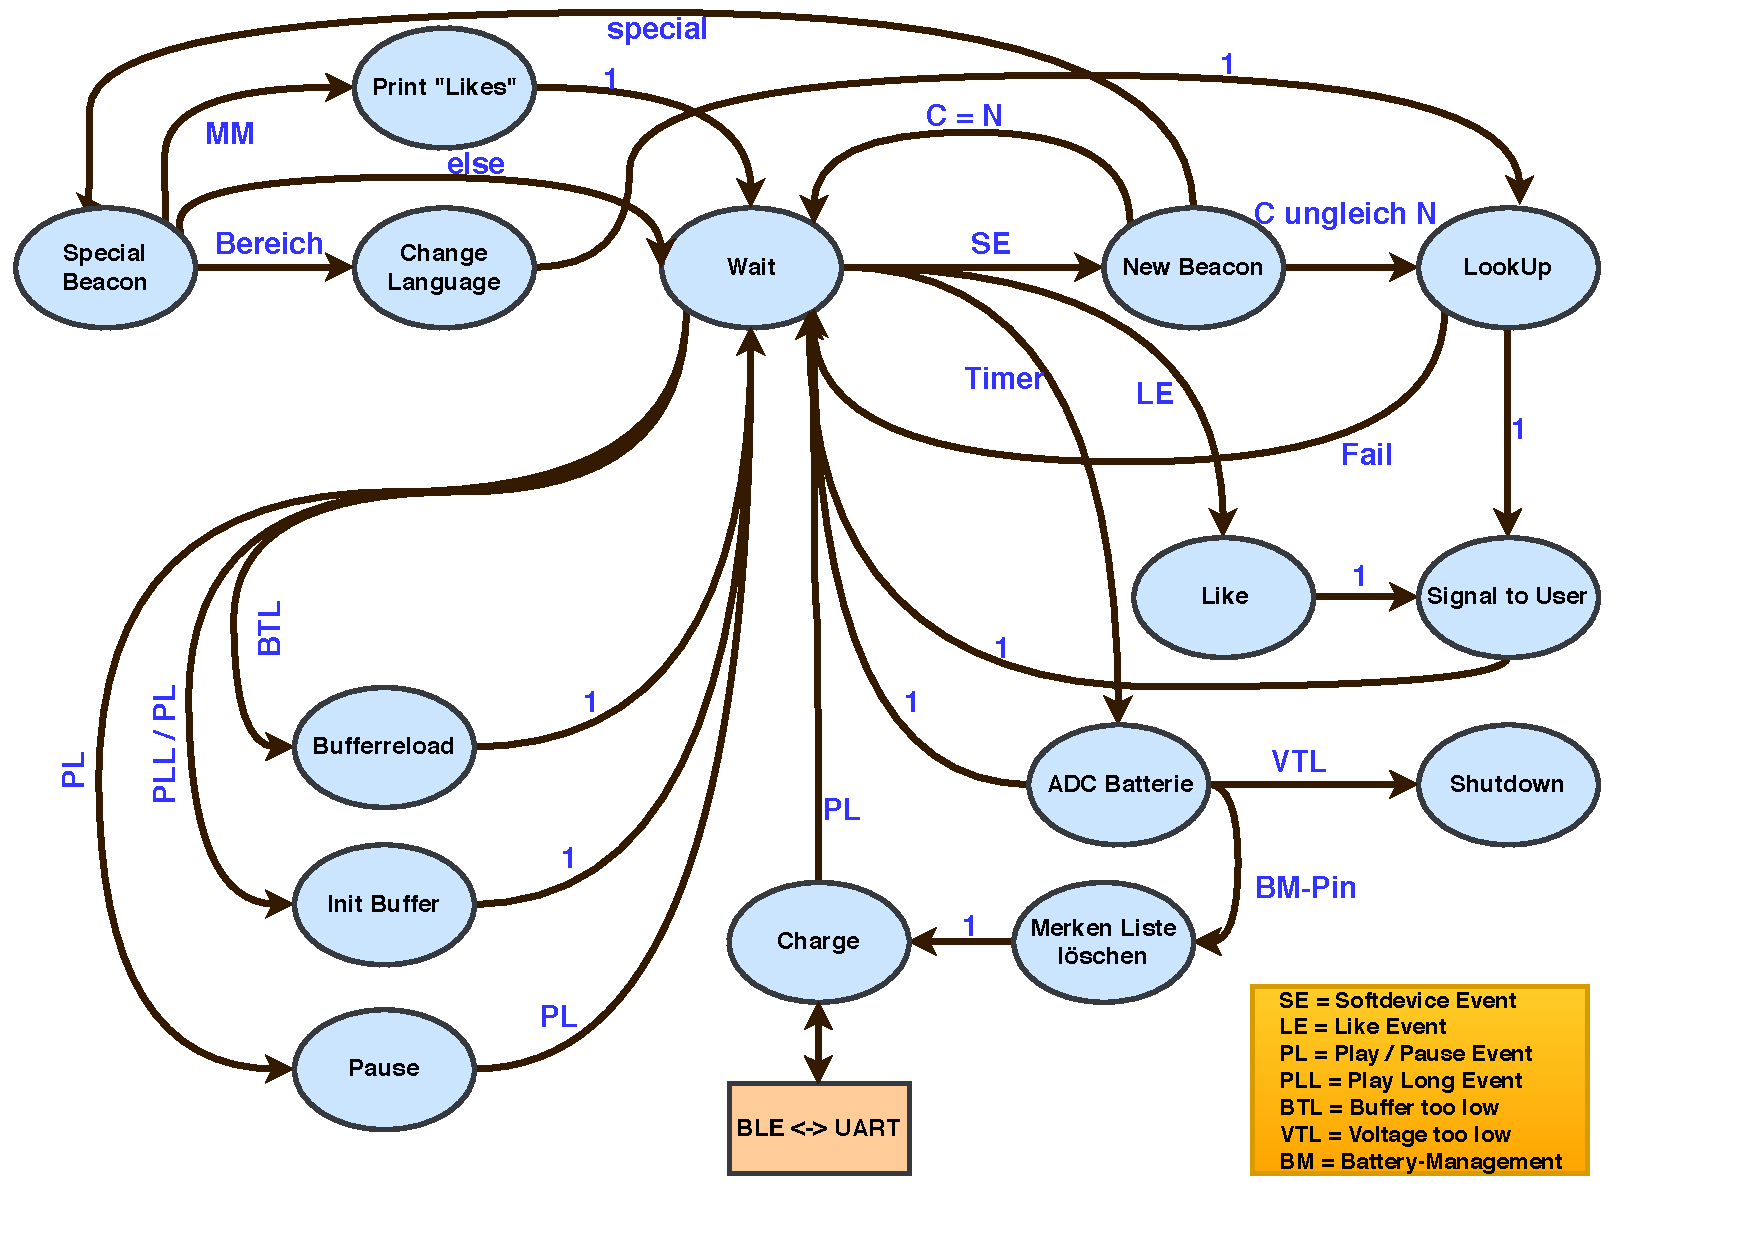
\includegraphics[width=1.15\textwidth]{Data/StateMachineFinal.pdf}
	\caption[Statemachine-Diagramm]{Statemachine im Überblick mit den einzelnen States und den Parametern}
	\label{fig:completeStateMachine}
\end{figure} 

\subsubsection*{State: Lookup}
In diesem State verschafft sich das Programm über die entsprechende Initialisierung Zugriff auf die SD-Karte der Anwendung. Falls der Mikrocontroller nicht auf die SD-Karte zugreifen kann, wird eine Fehlermeldung ausgegeben und die Funktion wird beendet. Anderenfalls wird dem Mikrocontroller signalisiert, dass der Zugriff geglückt ist und die eigentliche Funktion wird gestartet. Dazu werden die beiden Minor- und Majorzahlen in ein hexadezimales Zahlensystem gewandelt, welche dann als Vergleichskriterium verwendet werden. Falls die Nummer gefunden wird, kann das entsprechend zugehörige Audio-File über den Mikrocontroller ausgegeben werden. Verglichen wird jeweils zeilenweise, weshalb auch ein Fehlerhandling eingebaut wurde. Damit wird erkannt, ob sich das Textfile am Ende befindet. Somit lässt sich dann die Suche wiederholen, oder einen Fehler ausgeben. Die nachfolgende Abbildung \ref{fig:lookupState} zeigt den detaillierten Funktionsablauf im Lookup-State.

\begin{figure}[htbp!!!!]
	\centering
	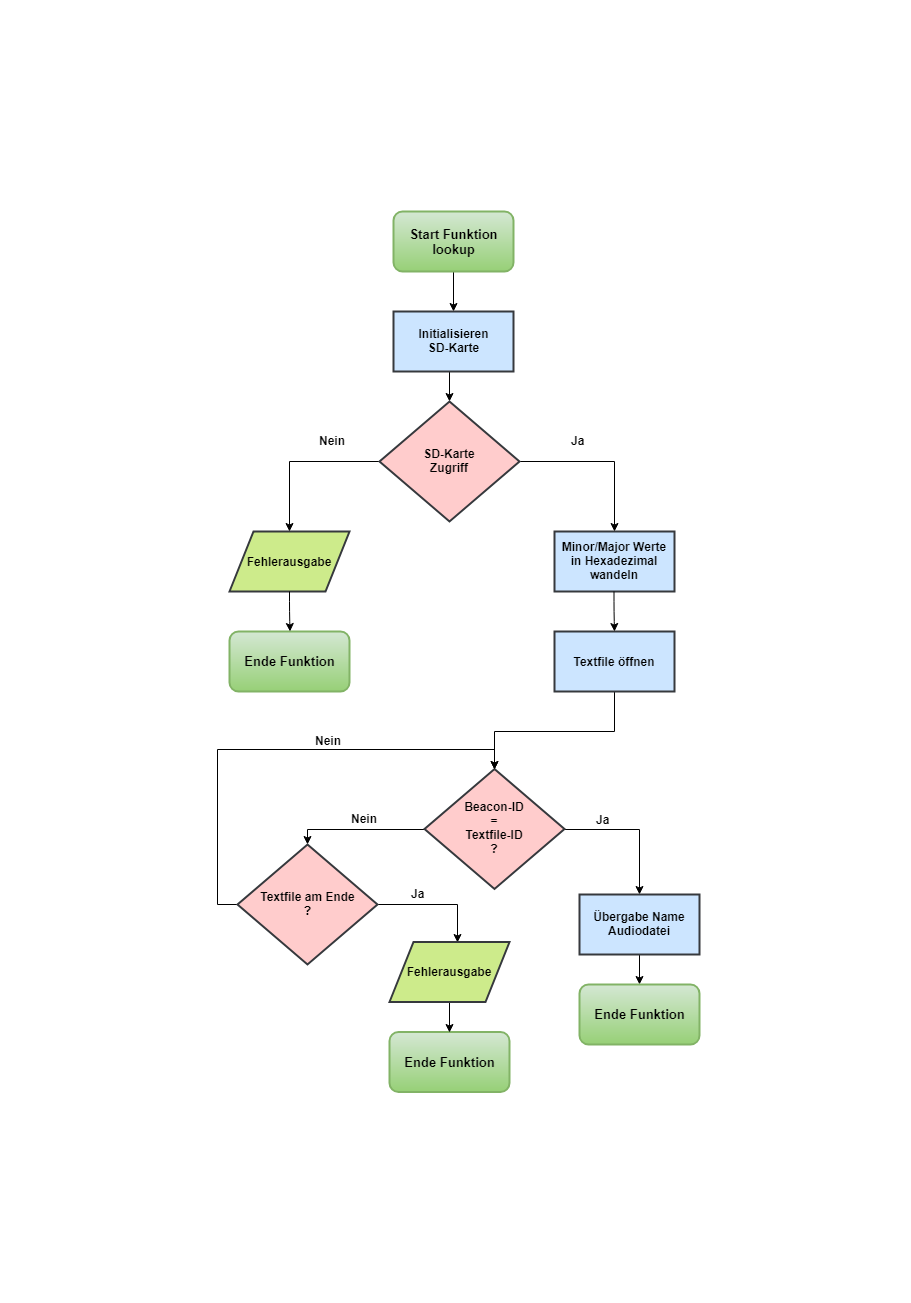
\includegraphics[width=0.57\textwidth]{Data/lookup_picture}
	\caption[Statemachine: lookup]{Funktionsablauf im lookup-State}
	\label{fig:lookupState}
\end{figure} 

\subsubsection*{State: Special Beacon}
Special Beacon dient hauptsächlich zur Unterscheidung der verschiedenen Beacons für die Sprache, das Drucken und weitere Features die in einem weiteren Ansatz implementiert werden können. Aus diesem Grund wurde dieser State auch relativ einfach gehalten. Zuerst wird verglichen, ob es sich dabei um die Sprachkonfiguration handelt. Ist dies zutreffend, so springt das Programm in den Change Language State. Anderenfalls wird überprüft, ob gerade der Like-Button gedrückt wird und entsprechend in den Print \glqq Likes \grqq State gewechselt wird. Ist keine der beiden Zustäde zutreffend, springt das Programm in den Wait State. Die nachfolgende Abbildung \ref{fig:specialBeaconState} zeigt den Ablauf der Funktion.

\begin{figure}[htbp!!!!]
	\centering
	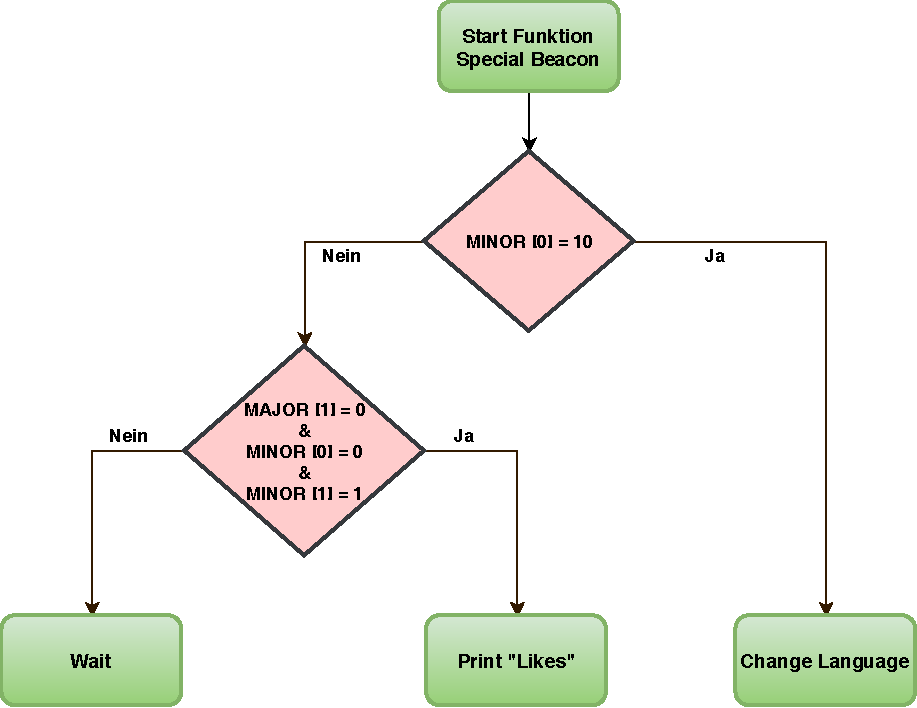
\includegraphics[width=0.9\textwidth]{Data/SpecialBeacon_picture.pdf}
	\caption[Statemachine: Special Beacon]{Funktionsablauf im Special Beacon State}
	\label{fig:specialBeaconState}
\end{figure} 
\newpage
\subsubsection*{State: Change Language}

Dieser State ist für die Sprachauswahl verantwortlich. Aufgrund des Zahlenwertes in Minor [1] wird zwischen den Landessprachen der Schweiz ausgewählt. Dabei wird die Vergleichstabelle in Form einer Datei kopiert und mit einem Kürzel entsprechend der Sprache versehen. Danach springt das Programm wieder in den lookup State.

\begin{figure}[htbp!!!!]
	\centering
	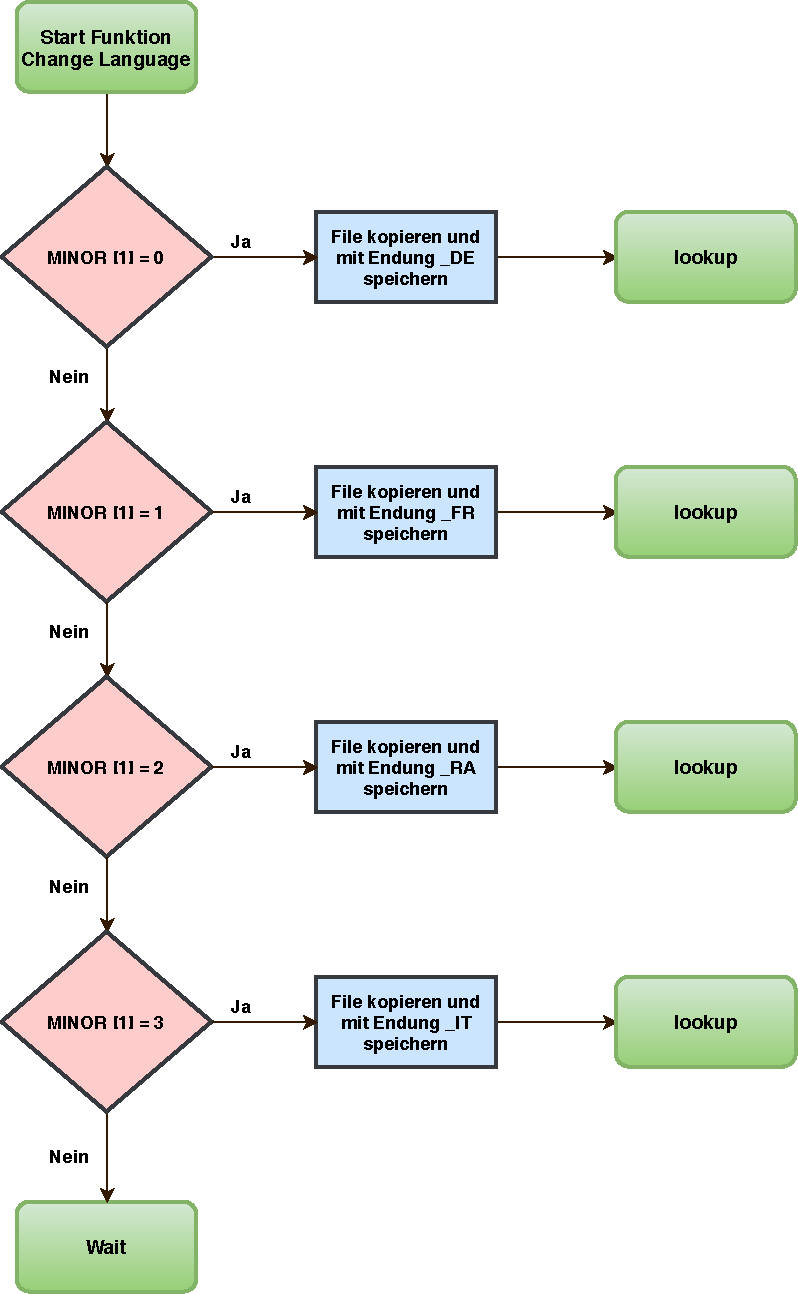
\includegraphics[width=0.7\textwidth]{Data/ChangeLanguage_picture.pdf}
	\caption[Statemachine: Change Language]{Funktionsablauf im Change Language State}
	\label{fig:changeLanguageState}
\end{figure} 

\subsubsection*{State: Print \glqq Likes \grqq}

Print \glqq Likes \grqq wurde nicht implementiert und das Hauptprogramm sprint in den Wait State. Das ist eine optionale Möglichkeit, die in einem weiteren Entwicklungskonzept bearbeitet werden kann. Die Software ermöglicht es aber diese Funktion noch einzubetten. Dabei könnte die Broschüre mit den interessanten Objekten direkt gedruckt werden und bereits für den Besucher am Ausgang des Museums bereit liegen.

\subsubsection*{State: Wait}



\subsubsection*{State: New Beacon}

\subsubsection*{State: Like}

\subsubsection*{State: Signal to User}

\subsubsection*{State: ADC Battery}

\subsubsection*{State: Shutdown}

\subsubsection*{State: Merken Liste löschen}

\subsubsection*{State: Charge}

\subsubsection*{State: Pause}

\subsubsection*{State: Init Buffer}

\subsubsection*{State: Bufferreload}